\documentclass{AeroStructure-ERJohnson}
\input crosslink.tex

%\usepackage{showframe}
\def\ShowFrameLinethickness{0.125pt}

%\def\harp#1{\smash{\mathord{\buildrel{\lower3pt\hbox{$\scriptscriptstyle\rightharpoonup$}}\over{#1}}}}

\allowdisplaybreaks

\myexternaldocument{App_4P}
\myexternaldocument{Ch01_4P}
\myexternaldocument{Ch02_4P}
\myexternaldocument{Ch03_4P}
\myexternaldocument{Ch04_4P}
\myexternaldocument{Ch05_4P}
\myexternaldocument{Ch06_4P}
\myexternaldocument{Ch07_4P}
\myexternaldocument{Ch08_4P}
\myexternaldocument{Ch09_4P}
\myexternaldocument{Ch10_4P}
\myexternaldocument{Ch11_4P}
\myexternaldocument{Ch12_4P}
%\myexternaldocument{Ch13_4P}
\myexternaldocument{Ch14_4P}
\myexternaldocument{Ch15_4P}
\myexternaldocument{Ch16_4P}
\myexternaldocument{Ch17_4P}
\myexternaldocument{Ch18_4P}

\begin{document}

\mainmatter

\setcounter{page}{345}
\setcounter{chapter}{12}

\chapter{Fracture of cracked\break members} \label{ch13}

The strength of ductile metals is limited by yielding. However, the presence of a crack in a structure may weaken it so that it fails by fracturing in two or more pieces. The study of crack propagation in bodies is the subject of \textbf{fracture mechanics}. Linear elastic fracture mechanics (\textbf{LEFM}) is the study of crack propagation in linear elastic bodies.

\textbf{Damage tolerant design} allows for the presence of subcritical cracks that will not grow to critical length between inspection intervals. Cracks can nucleate and grow in airplane structures under cyclic loading, or fatigue. This important structural issue of fatigue crack growth is tragically illustrated by the Comet disasters of 1954.

\section{Comet disasters of 1954}\label{sec13.1}

The content of this article is taken from Wikipedia, the free encyclopedia, and Cawthon (2005).

The\enlargethispage{-0.2\baselineskip} de Havilland Comet was the world's first commercial jet airliner to reach production. Developed and manufactured by de Havilland, it first flew in 1949 and was considered a landmark British aeronautical design. The Comet is an all-metal low-wing cantilever monoplane powered by four jet engines, approximately the length of a Boeing 737 but carrying fewer people in greater comfort. The clean, low-drag design featured many unique or innovative design elements, including a swept leading edge, integral wing fuel tanks, and four-wheel bogie main undercarriage units designed by de Havilland. The Comet was also the first pressurized jet-propelled commercial aircraft. Comet went into commercial service with BOAC on 22 January 1952. In May, the first paying passengers flew from Heathrow Airport to Johannesburg, South Africa. The Comet could fly higher and faster than any other airliner of the day and passengers loved it. They especially liked the Comet's big, rectangular windows, which allowed a much better view than those on competing planes. See figure~\ref{fig13.1}.

\begin{figure}\vspace*{-5pt}
\centering{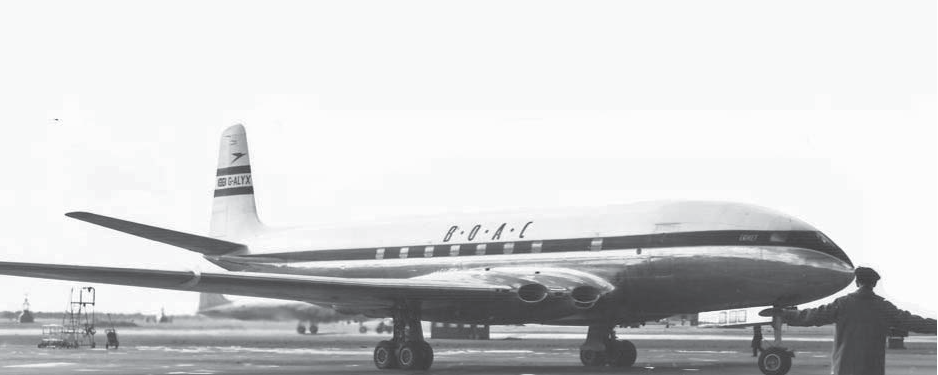
\includegraphics{Figure_13-1.pdf}}
\caption{BOAC De Havilland DH106 Comet 1G-ALYX on tarmac. (c) British Airways Speedbird Heritage Centre. Released under CC BY NC SA license 4.0.}\label{fig13.1}\vspace*{-7pt}
\end{figure}

The structural flaws in the Comet's design caused two fatal accidents in 1954. The first came just after the New Year, on January 10. BOAC Comet G-ALYP left Ciampino airport in Rome on its way to London. Less than a half-hour after takeoff, a routine radio call was cut off in mid-transmission. The Comet had crashed into the Mediterranean Sea about 16 miles from the island of Elba. The investigators determined the cabin failed because of metal fatigue. Just three months later, another Comet crashed, this time it was South African Airways G-ALYY, which was also flying out of Ciampino and also wound up in the Mediterranean, killing all twenty-one people on board. Authorities were unable to retrieve much wreckage, but cited the circumstances that caused the January incident.

Engineers subjected an identical airframe, G-ALYU (``Yoke Uncle''), to repeated repressurization and over pressurization and after 3,057 flight cycles (1,221 actual and 1,836 simulated), Yoke Uncle failed due to metal fatigue near the front port-side escape hatch. Investigators began considering fatigue as the most likely cause of both accidents, and further research into measurable strain on the skin began. Stress around the window corners was found to be much higher than expected, ``probably over 40,000 psi,'' and stresses on the skin were generally more than previously expected or tested. This was due to stress concentration, a consequence of the window's square shape. The stresses caused by thousands of takeoffs and landings were causing the plane's aluminum skin to begin to crack around the right-angle edges of those nice, big windows that were so popular with the passengers. Eventually the metal would completely fail, causing immediate depressurization of the cabin and catastrophic structure failure.

The problem was exacerbated by the punch rivet construction technique employed. The windows had been engineered to be glued and riveted, but had been punch riveted only. Unlike drill riveting, the imperfect nature of the hole created by punch riveting may cause the start of fatigue cracks around the rivet.

The square windows of the Comet 1 were redesigned as oval for the Comet 2, which first flew in 1953. The skin sheeting was thickened slightly. The remaining Comet 1s and 1As were either scrapped or modified with oval window rip-stop doublers. All production Comet 2s were modified to alleviate the fatigue problems, and most of these served with the Royal Air Force as the Comet C2. The Comet did not resume commercial airline service until 1958, when the much-improved Comet 4 was introduced and became the first jet airliner to enter transatlantic service. As is often the case in aeronautical engineering, other aircraft manufacturers learned from and profited by de Havilland's hard-learned lessons. Representatives from American manufacturers such as Boeing and Douglas ``admitted that if it hadn't been for our problems, it would have happened to one of them.''

The Comet 4 not only had a stronger airframe and rounded windows, it was also longer, carried more passengers, and had four new Rolls-Royce Avon engines, which produced twice the thrust of the original de Havilland Ghosts. BOAC had ordered nineteen of the new Comets in 1955, before the redesign was completed. The Comet 4 made its maiden flight on 27 April 1958 and de Havilland began delivering planes to BOAC in\vadjust{\vspace*{2pt}\pagebreak} September. BOAC started Comet passenger service with London to New York on 4 October 1958, beating Pan Am's inaugural 707 Clipper Service by three weeks.

But it was too late. The Comet, unbeatable in 1954, was an also-ran in 1958. In addition to its early problems, the Comet's dated design and smaller size convinced most carriers to select the newer 707 or Douglas DC-8. Only seventy-six Comet 4s were built from 1958 to 1964, and it was America, not Great Britain, that owned the commercial jetliner market for the rest of the twentieth century.

\section{Cracks as stress raisers}\label{sec13.2}

Some of the discussion in this article paraphrases that given by Dowling (1993, p.279). Consider the linear elastic response of a rectangular plate containing a centrally located elliptical hole that is subject to a remote tensile stress $\sigma$. See figure~\ref{fig13.2}. The major axis of the through hole is denoted by $a$ and the minor axis by $d$. The radius of curvature $\rho$ at the tip of the major axis is given by $\rho=d^{2}/a$.

\processfigure{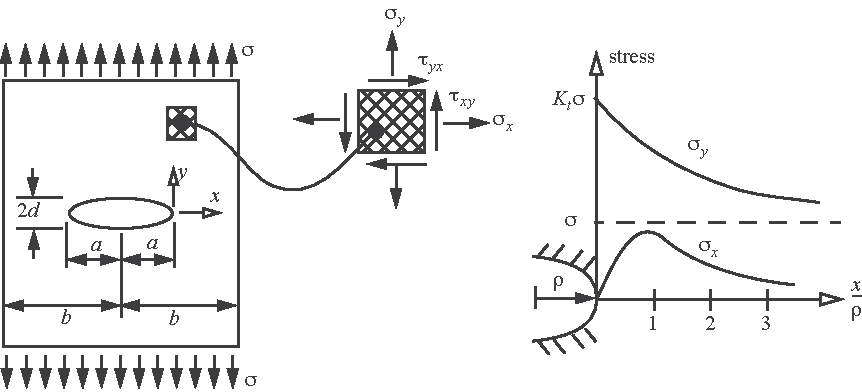
\includegraphics{Figure_13-2.pdf}}{\caption{Stresses at the tip of an elliptical through hole in a rectangular plate subject to remote tension.}\label{fig13.2}}

The stress concentration factor, $K_{t}$, at the edge of the hole is defined by
\begin{align}\label{eq13.1}
K_{t}=\frac{\left.\sigma_{y}(x, y)\right|_{x=y=0}}{\sigma}.
\end{align}
From linear elasticity for a plate half width $b \gg a$, this stress concentration factor for an isotropic material is given~by
\begin{align}\label{eq13.2}
K_{t}=1+2 \frac{a}{d}=1+2 \sqrt{\frac{a}{\rho}}.
\end{align}
For selected values of the ratio \textit{a/d, }the stress concentration factors are listed in table~\ref{tab13.1}.

\begin{table}
\processtable{Stress concentration factors for selected elliptical hole sizes \label{tab13.1}}{%
\tabcolsep=60pt\begin{tabular}{@{}ll@{}}
\toprule
\colhead{$a/d$} & \colhead{$K_{t}$} \\
\midrule
1 (circular hole) & 3 \\
2 & 5 \\
3 & 7 \\
\botrule
\end{tabular}}{}
\vspace*{-1pc}
\end{table}

As $d\rightarrow 0$, or $\rho\rightarrow 0$, $K_{t}\rightarrow \infty$. This limiting geometry is a crack-like slit. Consequently the plate experiences a strength failure at no load. Clearly, this is a theoretical result from linear elasticity. Real materials\vadjust{\vspace*{6pt}\pagebreak} cannot support infinite stress. In ductile metals, large plastic deformation exists in the vicinity of the crack tip. The stress is not infinite and the sharp crack tip is blunted.

There are generally three modes of loading, which involve different crack surface displacements as depicted in the sketches of figure~\ref{fig13.3}. The three modes are:\vspace*{-6.9pt}
\begin{description}
\item[Mode I:] opening or tensile mode (the crack faces are pulled apart)
\item[Mode II:] sliding or in-plane shear (the crack surfaces slide over each other)
\item[Mode III:] tearing or anti-plane shear (the crack surfaces move parallel to the leading edge of the crack and relative to each other)
\end{description}

\vspace*{-12pt}

\processfigure{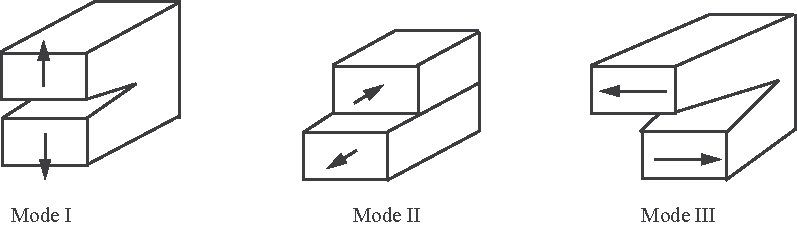
\includegraphics{Figure_13-3.pdf}}{\caption{Basic displacement modes of a cracked body.}\label{fig13.3}}

\vspace*{-1pc}

\section{LEFM stress field in the vicinity of the crack tip for mode I}\label{sec13.3}

A center-cracked plate subject to remote tension, or mode I loading, is shown in figure~\ref{fig13.4}. This loading is symmetric with respect to the crack surface. The crack length is 2$a$, plate width 2$b$, and the plate thickness $t$. The two free surface areas of the crack are 2$a$-by-$t$. The remote tensile stress is denoted by $\sigma$. Let $r$ and $\theta$ denote the polar coordinates in the \textit{x-y} plane measured from the crack tip. From linear elastic fracture mechanics (Anderson, 1995, pp. 31--96), LEFM, the dominant terms in the stress field near the crack tip are as follows:
\begin{gather}
\sigma_{x}=\frac{K_{I}}{\sqrt{2 \pi r}} \cos \frac{\theta}{2}\left[1-\sin \frac{\theta}{2} \sin \frac{3 \theta}{2}\right]+\ldots, \label{eq13.3} \\
\sigma_{y}=\frac{K_{I}}{\sqrt{2 \pi r}} \cos \frac{\theta}{2}\left[1+\sin \frac{\theta}{2} \sin \frac{3 \theta}{2}\right]+\ldots, \label{eq13.4} \\
\tau_{x y}=\frac{K_{I}}{\sqrt{2 \pi r}} \cos \frac{\theta}{2} \sin \frac{\theta}{2} \cos \frac{3 \theta}{2}+\ldots, \label{eq13.5} \\
\nonumber\\
\sigma_{z}=\left\{\begin{array}{@{}c@{}}0, \text { plane stress where } \varepsilon_{z} \neq 0 \\[6pt]
v\left(\sigma_{x}+\sigma_{y}\right), \text { plane strain where } \varepsilon_{z}=0\end{array}\right., \label{eq13.6} \\
\tau_{z x}=\tau_{z y}=0. \label{eq13.7}
\end{gather}
Poisson's ratio is denoted by $v$. The plane stress solution is more appropriate if the thickness $t$ is relatively small, and the plane strain solution is more appropriate if the thickness is relatively large. At $\theta=0$, stress components $\sigma_{x}=\sigma_{y} \approx \frac{K_{I}}{\sqrt{2 \pi r}}$ near $r \approx 0$. So $\sigma_{x} \text { and } \sigma_{y} \rightarrow \infty$ as $r \rightarrow 0$. For small values of \textit{r}, stress components $\sigma_{x}$ and $\sigma_{y}$ are proportional to $K_{I}$.

\processfigure{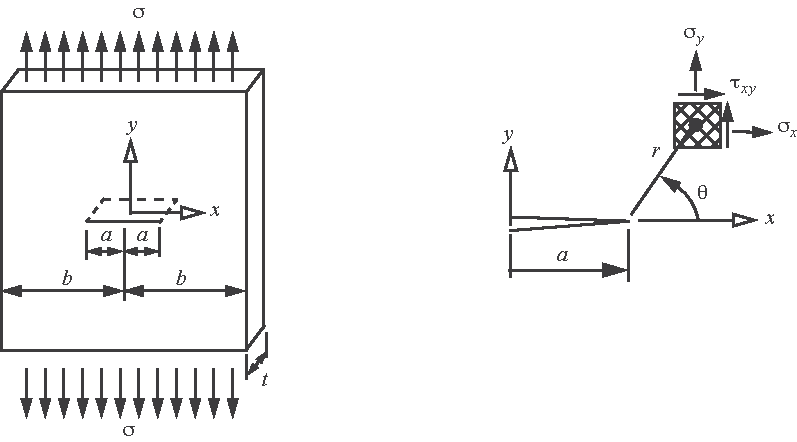
\includegraphics{Figure_13-4.pdf}}{\caption{Mode I loading of a center-cracked plate.}\label{fig13.4}}

The magnitude of the stress field in the vicinity of the crack tip is characterized by $K_{I}$. Hence, $K_{I}$ is a measure of the severity of the crack. \textbf{The parameter $K_{I}$ is called the mode I stress intensity factor}. For an infinite plate, where $b \rightarrow \infty$ with $a>0$, LEFM yields the result that
\begin{align}\label{eq13.8}
K_{I}=\sigma \sqrt{\pi a}.
\end{align}
For finite plate geometries
\begin{align}\label{eq13.9}
K_{I}=F \sigma \sqrt{\pi a},
\end{align}
where \textit{F} is a dimensionless width-correction factor that is a function of the geometry and the ratio of \textit{a/b. }For the center-cracked plate, the quantity \textit{F} is given by
\begin{align}
F=\left\{\begin{array}{@{}c@{}}\frac{1\,-\,0.5(a / b)\,+\,0.326(a / b)^{2}}{\sqrt{1-(a / b)}} \\1 \quad a / b \leq 0.4\end{array}\right. , \textrm{ and} \label{eq13.10} \\
F=1 \text { if } 0<\frac{a}{b} \ll 1. \label{eq13.11}
\end{align}
In general the correction factor is a function of the loading configuration as well as the geometry and ratio of\textit{ a/b}. The reader is referred to Dowling (1999) and the references cited there for additional relations for \textit{F}.

The following facts are noted:
\begin{itemize}
\item The mode I stress intensity factor $K_{I}$ depends on the remote stress $\sigma$, and $\sigma$ is the stress $\sigma_{y}$ if \textbf{no} crack is present.
\item The mode I stress intensity factor $K_{I}$ depends on the square root of the half crack length.
\item The dimensional units of $K_{I}$ are stress times the square root of length (e.g., $\mathrm{ksi} \sqrt{\mathrm{in}}$ in U.S. customary units, or $\mathrm{MPa} \sqrt{\mathrm{m}}$ in SI units.)
\end{itemize}

\begin{figure}[!h]
\centerline{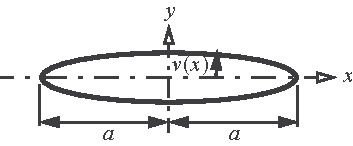
\includegraphics{Figure_13-5.pdf}}
\caption{Opening displacement of the crack under mode I loading of the center-cracked plate.} \label{fig13.5}
\end{figure}

The crack opening displacement $v(x)$ along the crack surface is also of interest, where the origin of the $x$-axis is located at the center of the crack as is shown in figure~\ref{fig13.7}. For the infinite plate geometry under mode I loading, the displacement at the upper and lower crack faces are symmetrical, so only the displacement on the upper crack surface needs to be described. The expression for $v(x)$ as given by Sun (1998, p. 162) is
\begin{align}\label{eq13.12}
v(x)=\frac{(\kappa+1)(1+v)}{2 E} \sigma \sqrt{a^{2}-x^{2}} \quad|x| \leq a,
\end{align}
where
\begin{align}\label{eq13.13}
\kappa=\left\{\begin{array}{@{}l@{}}3-4 v \text { for plane strain } \\[6pt]
\frac{3-v}{1+v} \text { for plane stress }\end{array}\right..
\end{align}

\subsubsection{The critical mode I stress intensity factor is denoted by $\textbf{\textit{K}}_{\textbf{\textit{Ic}}}$, and it is assumed to be a material parameter.}
\begin{itemize}
\item $K_{I}<K_{I c}$. There is no crack growth, and the material resists the crack without brittle fracture.
\item $K_{I}=K_{I c}$. The crack begins to propagate and brittle fracture occurs.
\end{itemize}
The critical mode I stress intensity factor is also called the \textbf{fracture toughness}. A tough material has a large value of $K_{I c}$, which means it is effective in resisting crack growth. At crack growth, the remote stress is denoted by $\sigma_{\mathrm{cr}}$ and is given by
\begin{align}\label{eq13.14}
\sigma_{\mathrm{cr}}=\frac{K_{I c}}{F \sqrt{\pi a}}.
\end{align}
A representative graph of eq.~(\ref{eq13.14}) is shown in figure~\ref{fig13.6}. The value of the half crack length when $\sigma_{c r}=\sigma_{Y}$, is called the transition crack length $a_{t}$, where $\sigma_{Y}$ denotes the yield strength of the material. Set $\sigma_{\mathrm{cr}}=\sigma_{Y}$\vadjust{\vspace*{6pt}\pagebreak} in eq.~(\ref{eq13.14}) to\vspace*{-10pt} find

\processfigure[!h]{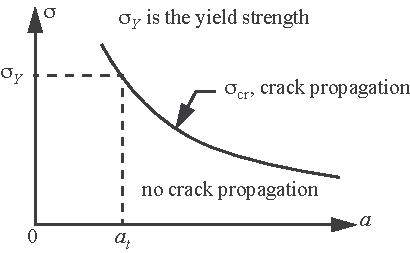
\includegraphics{Figure_13-6.pdf}}{\caption{Representative graph of the critical stress\break for crack propagation as a function of the half crack\break length.}\label{fig13.6}}

\vspace*{-1.8pc}

\begin{align}\label{eq13.15}
a_{t}=\frac{1}{\pi}\left(\frac{K_{I c}}{\sigma_{Y}}\right)^{2}.
\end{align}
The transition crack length is the approximate length above which strength is limited by fracture. If $a>a_{t}$ then fracture limits strength. If $a<a_{t}$ then yielding dominates strength. Materials with
\begin{enumerate}
\item[a.] high $K_{I c}$ and low $\sigma_{Y}$ imply a long $a_{t}$ and small cracks are no problem, and
\item[b.] low $K_{I c}$ and high $\sigma_{Y}$ imply a short $a_{t}$ and small cracks can be a problem.
\end{enumerate}


Typical values of the fracture toughness at room temperature are listed in table~\ref{tab13.2}.

\begin{table}[!h]
\processtable{Fracture toughness and corresponding tensile properties for selected metals at room temperature (Dowling, 1999). \label{tab13.2}}{%
\tabcolsep=12pt\begin{tabular}{@{}lllllll@{}}
\toprule
 & \multicolumn{2}{c}{\colhead{Toughness $K_{I c}$}} & \multicolumn{2}{c}{\colhead{Yield strength $\sigma_{Y}$}} & \multicolumn{2}{c}{\colhead{Ultimate Strength $\sigma_{U}$}} \\[-5pt]
 & \multicolumn{2}{c}{\hrulefill} & \multicolumn{2}{c}{\hrulefill} & \multicolumn{2}{c}{\hrulefill} \\
\colhead{Material} & \colhead{$\mathrm{MPa}\sqrt{\mathrm{m}}$} & \colhead{$\mathrm{ksi}\sqrt{\mathrm{in}}$} & \colhead{MPa} & \colhead{ksi} & \colhead{MPa} & \colhead{ksi} \\
\midrule
\multicolumn{7}{@{}l}{\textit{Steels}} \\
AISI 1144 & \phantom{0}66 & \phantom{0}60 & \phantom{0}540 & \phantom{0}78 & \phantom{0}840 & 122 \\
AISI 4130 & 110 & 100& 1090& 158& 1150& 167 \\[6pt]
\multicolumn{7}{@{}l}{\textit{Aluminum and titanium alloys (L-T Orientation)}} \\
2014-T651 &  \phantom{0}24 &  \phantom{0}22 &  \phantom{0}415 &  \phantom{0}60 &  \phantom{0}485 &  \phantom{0}70 \\
2024-T351 &  \phantom{0}34 &  \phantom{0}31 &  \phantom{0}325 &  \phantom{0}47 &  \phantom{0}470 &  \phantom{0}68\\
2219-T851 &  \phantom{0}36 &  \phantom{0}33 &  \phantom{0}350 &  \phantom{0}51 &  \phantom{0}455 &  \phantom{0}66\\
7075-T651 &  \phantom{0}29 &  \phantom{0}26 &  \phantom{0}505 &  \phantom{0}73 &  \phantom{0}570 &  \phantom{0}83\\
7475-T7351 &  \phantom{0}52 &  \phantom{0}47 &  \phantom{0}435 &  \phantom{0}63 &  \phantom{0}505 & \phantom{0}73\\
Ti-6Al-4V annealed &  \phantom{0}66 &  \phantom{0}60 &  \phantom{0}925 &  134 &  1000 &  145\\
\botrule
\end{tabular}}{}
\vspace*{-1.5pc}
\end{table}

\begin{example}[ASTM compact tension configuration]\label{ex13.1}The configuration shown in figure~\ref{fig13.7} is subject to a tensile load \textit{P}, has a crack length denoted by $a$, and a thickness denoted by $t$. It is the configuration of the ASTM standard compact specimen. The mode I stress intensity factor is given by (Dowling, p. 295\vadjust{\vspace*{6pt}\pagebreak})

\begin{equation}
K=F_{P}(\alpha) \frac{P}{t \sqrt{b}}, \label{eq13.1.a}\tag{a}
\end{equation}

\vspace*{-1pc}

\begin{wrapfigure}[6]{L}{72pt}
\vspace{-5pc}
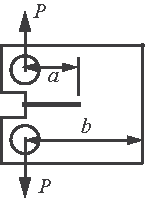
\includegraphics{Figure_13-7.pdf}
\caption{ \label{fig13.7}}
\end{wrapfigure}

\noindent where $\alpha=a/b$. The nondimensional function $F_p$ is
\begin{equation}
F_{p}(\alpha)=\frac{(2+\alpha)}{(1-\alpha)^{3 / 2}}\left[0.866+4.64 \alpha-13.32 \alpha^{2}+14.72 \alpha^{3}-5.6 \alpha^{4}\right] \quad \alpha \geq 0.2. \label{eq13.1.b}\tag{b}
\end{equation}

For $P=22 \textrm{~kN}$, $b= 50$ mm, and $t= 25$ mm, determine the critical crack length for brittle fracture of 2024-T351 aluminum alloy. The numerical factor multiplying $F_p$ is
\begin{equation}
\frac{P}{t \sqrt{b}}=\frac{22{,}000 \mathrm{~N}}{25 \mathrm{~mm} \sqrt{50 \mathrm{~mm}\left(10^{3} \mathrm{~mm} / \mathrm{m}\right)}}=\frac{22{,}000}{25 \sqrt{50{,}000}}\left(\frac{\mathrm{N}}{\mathrm{mm}^{2}}\right) \sqrt{\mathrm{m}}=3.93548 \textrm{ MPa} \sqrt{\mathrm{m}}. \label{eq13.1.c}\tag{c}
\end{equation}
A graph of the stress intensity factor as a function of the crack length in the range from 15~mm to 35~mm is shown in figure~\ref{fig13.8}. The critical mode I stress intensity factor is 34~MPa $\sqrt{\mathrm{m}}$ from table~\ref{tab13.2}, and it plots as horizontal line in the graph. Using a root finding procedure, or a trial and error method, the intersection of the two lines in the graph occurs at 23.1~mm. Thus, the critical crack length for brittle fracture is 23.1~mm.
\end{example}

\processfigure{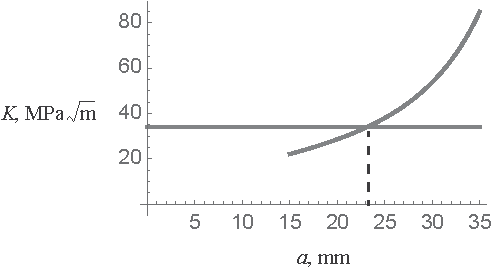
\includegraphics{Figure_13-8.pdf}}{\caption{Stress intensity factor as a function of crack length.}\label{fig13.8}}

The example that follows illustrates how the methods of strength of materials and fracture mechanics are employed to analyze the strength of a cantilever beam.

\begin{example}[Strength of a cantilever beam.]\label{ex13.2}This example is adapted from Kanninen and Popelar (1985, pp. 10--12). Determine the maximum value of the tip load $Q$ acting on a cantilever beam depicted in figure~\ref{fig13.9} by the strength of materials method and the fracture mechanics method. The beam has a length $L=300 \mathrm{~mm}$, height $h=30 \mathrm{~mm}$, and rectangular cross section with width $b=15 \mathrm{~mm}$. Assume a factor of safety (FS) of 1.5. The material is aluminum alloy 2014-T651 with properties listed in table~\ref{tab13.2}. Plot the maximum value of \textit{Q} versus the crack length $a$.

\processfigure{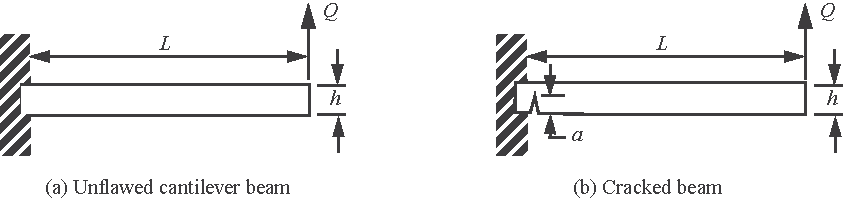
\includegraphics{Figure_13-9.pdf}}{\caption{Basis for the comparison of strength of materials and fracture mechanics approaches.}\label{fig13.9}}

\subsubsection{(a) Strength of materials approach.} The maximum load is determined such that the maximum stress in the beam is less than the yield strength of the material. The maximum tensile normal stress occurs at the bottom\pagebreak\ of\break the beam at its built-in end. The bending moment at the built-in end is $M=L Q$, and the flexure formula for the maximum normal stress is
\begin{equation}
\sigma_{\max }=\frac{M(h / 2)}{I}, \label{eq13.2.a}\tag{a}
\end{equation}
where the second area moment of the rectangular cross section is $I=\left(b h^{3}\right) / 12$. Hence,
\begin{equation}
\sigma_{\max }=\frac{6 Q L}{b h^{2}}<\frac{\sigma_{Y}}{F S}. \label{eq13.2.b}\tag{b}
\end{equation}
Solve the inequality for the load in eq. (\textbf{\ref{eq13.2.b}}) to get
\begin{equation}
Q<\frac{b h^{2}}{6(F S) L} \sigma_{Y}=\frac{(15 \mathrm{~mm})(30 \mathrm{~mm})^{2}}{6(1.5)(300 \mathrm{~mm})}(415 \mathrm{~N} / \mathrm{mm}^{2}). \label{eq13.2.c}\tag{c}
\end{equation}
Hence, $Q<2075 \mathrm{~N}$.

\subsubsection{(b) Fracture mechanics approach.} Consider that the beam, instead of being defect free, contains an edge crack of length $a$ normal to the free edge. Further suppose that, as shown in figure~\ref{fig13.9}(b), the crack is located where the maximum tensile stress is anticipated. This geometry and loading configuration is not the center-cracked plate. However, for a relatively small crack, an LEFM-based analysis of the flawed beam shown in figure~\ref{fig13.9}(b) would give a reasonable approximation in the following expression for the stress intensity factor:
\begin{equation}
K_{I}=1.12 \sigma_{\max } \sqrt{\pi a}, \label{eq13.2.d}\tag{d}
\end{equation}
where $\sigma_{\max }$ is the stress that would occur at the crack location \textit{in the absence of the crack}. The beam is safe from fracture if $K_{I} \leq K_{I c}$. Further assurance can be obtained by having $K_{I}<K_{I c} /(F S)$, where, just as in the strength of materials approach, the number \textit{FS} is the factor of safety. Using eq. (\textbf{\ref{eq13.2.b}}) to replace $\sigma_{\max }$ in eq. (\textbf{\ref{eq13.2.d}}) then leads to
\begin{equation}
K_{I}=1.12\left(\frac{6 Q L}{b h^{2}}\right) \sqrt{\pi a}<\frac{K_{I c}}{\textit{FS}}. \label{eq13.2.e}\tag{e}
\end{equation}
Solve eq. (\textbf{\ref{eq13.2.e}}) for the load to get
\begin{equation}
Q<\left(\frac{b h^{2}}{6(\textit{FS}) L}\right) \frac{K_{I c}}{1.12 \sqrt{\pi a}}. \label{eq13.2.f}\tag{f}
\end{equation}
Substitute numerical values into eq. (\textbf{\ref{eq13.2.f}}) to get
\begin{equation}
Q<\left[\frac{(15 \mathrm{~mm})(30 \mathrm{~mm})^{2}}{6(1.5)(300 \mathrm{~mm})}\right] \frac{\left(24 \mathrm{~N} / \mathrm{mm}^{2}\right) \sqrt{\mathrm{m}\left(10^{3} \mathrm{~mm} / \mathrm{m}\right)}}{1.12 \sqrt{\pi a}}. \label{eq13.2.g}\tag{g}
\end{equation}
\vspace*{2pt}
\pagebreak

\noindent Hence, $Q<\frac{1911.56 \mathrm{~N} \sqrt{\mathrm{mm}}}{\sqrt{a}}$, which is the fracture mechanics estimate of the safe operating load. A graph of the failure load is shown in figure~\ref{fig13.10}. From the plots in the graph, yielding governs failure for $0<a<0.849 \mathrm{~mm}$, whereas fracture governs failure for $a>0.849 \mathrm{~mm}$. The transition crack length, $a_{t}=0.849 \mathrm{~mm}$, determines the crack length for which it can be expected that fracture rather than yielding governs the mode of failure. In this example the transition crack length is only 2.8 percent of the height, $h$, of the beam.

\begin{figure}[!h]
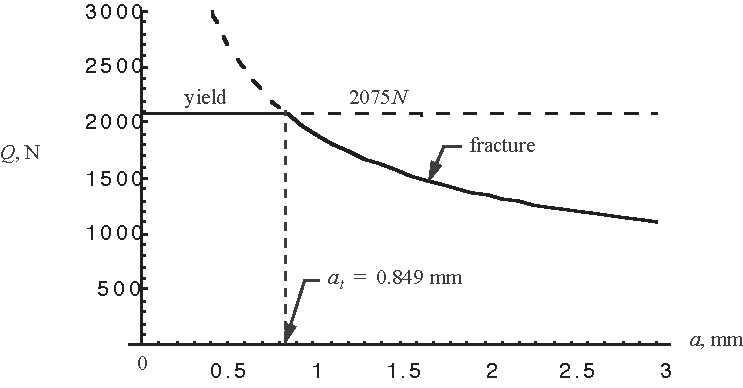
\includegraphics{Figure_13-10.pdf}
\caption{Failure load versus crack length for the cantilever beam of example~\ref{ex13.2}.} \label{fig13.10}
\end{figure}

A comparison between eq. (\textbf{\ref{eq13.2.c}}) and eq. (\textbf{\ref{eq13.2.g}}) is instructive. It can be seen that the structural geometry and the factor of safety enter both relations in exactly the same way – that is, through the multiplicative parameter $\left(b h^{2}\right) /(6(F S) L)$. Also, both relations contain a basic, albeit different, material property. The essential difference is that the fracture mechanics approach explicitly introduces a new physical parameter: the size of a (real or postulated) crack-like flaw. In fracture mechanics the size of the crack is the dominant structural parameter. It is the specification of this parameter that distinguishes fracture mechanics from conventional failure analyses.
\end{example}

\vspace*{-1pc}

\section{LEFM stress field in the vicinity of the crack tip for mode II}\label{sec13.4}

Mode II fracture is associated with loading that is antisymmetric with respect to the crack surface. Shear loading is shown in figure~\ref{fig13.11} and is a mode II fracture problem.

\vspace*{-6pt}

\processfigure{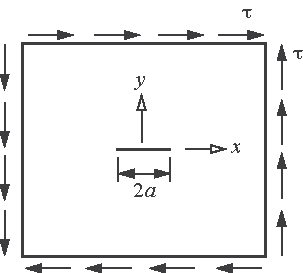
\includegraphics{Figure_13-11.pdf}}{\caption{Antisymmetric shear loading.}\label{fig13.11}}
\vspace*{5pt}
\pagebreak

From the linear elastic fracture mechanics analysis, the singular stress field near the crack tip in terms of the polar coordinates shown in figure~\ref{fig13.4} is
\begin{gather}
\sigma_{x}=-\left(\frac{K_{I I}}{\sqrt{2 \pi r}}\right) \sin \frac{\theta}{2}\left[2+\cos \frac{\theta}{2} \cos \frac{3 \theta}{2}\right]+\ldots, \label{eq13.16} \\
\sigma_{y}=\frac{K_{I I}}{\sqrt{2 \pi r}} \sin \frac{\theta}{2} \cos \frac{\theta}{2} \cos \frac{3 \theta}{2}+\ldots, \label{eq13.17}
\\
\tau_{x y}=\frac{K_{I I}}{\sqrt{2 \pi r}} \cos \frac{\theta}{2}\left(1-\sin \frac{\theta}{2} \sin \frac{3 \theta}{2}\right)+\ldots, \label{eq13.18}
\end{gather}
where $K_{II}$ is the mode II stress intensity factor, and $r=0$ at the crack tip. Along the $x$-axis where $\theta=0$, the stresses near the crack tip are\vspace*{-0.6pc}
\begin{align}\label{eq13.19}
\sigma_{x}=\sigma_{y}=0 \quad \tau_{x y}=\frac{K_{I I}}{\sqrt{2 \pi r}}+\ldots.
\end{align}
Hence, the linear elastic analysis gives $\tau_{x y} \rightarrow \infty$ as $r \rightarrow 0$. For an infinite plate subject to a uniform shear $\tau$ as shown in figure~\ref{fig13.11},
\begin{align}\label{eq13.20}
K_{I I}=\tau \sqrt{\pi a}\quad \textrm{ LEFM infinite plate solution.}
\end{align}

\subsubsection{The critical mode II stress intensity factor is denoted by $\textbf{\textit{K}}_{\textbf{\textit{IIc}}}$, and it is assumed to be a material parameter.}
\begin{itemize}
\item $K_{I I}<K_{I I c}$. There is no crack growth, and the material resists the crack without brittle fracture.
\item $K_{I I}=K_{I I c}$. The crack begins to propagate and brittle fracture occurs.
\end{itemize}
The critical mode II stress intensity factor is also called the \textbf{mode II} \textbf{fracture toughness}.

The displacements on the two crack surfaces are antisymmetric with respect to the $x$-axis. Let $u$ denote the displacement component in the $x$-direction, and let $v$ denote the displacement component in the $y$-direction. The expression for the upper surface displacement $u(x)$ as given by Sun (1998, p. 163) is
\begin{align}\label{eq13.21}
u=\frac{(\kappa+1)(1+v)}{2 E} \tau \sqrt{a^{2}-x^{2}} \textrm{ and } v(x)=0, |x| \leq a.
\end{align}
The origin of the $x$-axis is located at the center of the crack as is shown in figure~\ref{fig13.5}, and $\kappa$ depends on Poisson's ratio, which is given by eq.~(\ref{eq13.13}). Under antisymmetric loading the crack surfaces are in sliding contact with each other and do not open as they do in mode I.

\section{Energy criterion for crack growth}\label{sec13.5}

The text that follows is taken from Gordon (1978).

\begin{quote}
The paradox that a material with a sharp crack has infinite stress at the tip, so that it fails at infinitesimal load, motivated Griffith to develop a fracture theory based on energy.

From chemistry, the surface energy needed to break chemical bonds on any one plane is from 0.1 to 1.0 J/m$^{2}$ for most structural solids. For brittle materials – stone, brick, concrete – 1 J/m$^{2}$ is nearly all the energy,\vadjust{\vspace*{6pt}\pagebreak} or work, required to produce a new fracture surface. Ductile materials – many metals – yield before fracture, so much work goes into plastic deformation ahead of the crack tip. Some approximate values of the work of fracture are listed in the table [table~\ref{tab13.3}] that follows.

A tough material has a work of fracture between 10$^{3}$--10$^{6}$~J/m$^{2}$.
\end{quote}

\begin{table}[!h]
\processtable{Work of fracture for selected materials from Gordon (1978) \label{tab13.3}}{%
\tabcolsep=12pt\begin{tabular}{@{}lll@{}}
\toprule
 & \colhead{Approximate work} & \colhead{Approximate tensile} \\
\colhead{Material} & \colhead{of fracture J/m$^{\textbf{2}}$} &  \colhead{strength MPa} \\
\midrule
glass, pottery & 1--10 & 170 \\
cement, brick & 3--40 & 4 \\
epoxy resins & 100 & 50 \\
wood & 10,000 & 100 \\
mild steel & 10$^{4}$--10$^{6}$ & 4,000 \\
high tensile steel & 10$^{4}$ & 1,000 \\
\botrule
\end{tabular}}{}
\vspace*{-1.5pc}
\end{table}

\subsection{Griffith criterion}\label{sec13.5.1}

The rationale for the Griffith energy criterion is the first law of thermodynamics and the theorem of minimum potential energy for an elastic body. The critical condition for equilibrium crack growth is that there is no net change in the total energy (Anderson, 1995, p. 36). Consider a cracked plate of thickness $t$ with a through crack of length $a$ as shown in figure~\ref{fig13.12}. Then the infinitesimal increase in the crack area is $d A=t d a$.

\vspace*{-5pt}

\processfigure{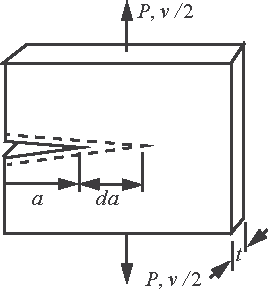
\includegraphics{Figure_13-12.pdf}}{\caption{Mode I loading of a cracked plate.}\label{fig13.12}}

\vspace*{-5pt}

\noindent Let \textit{E} denote the total energy, $U$ the total strain energy contained in the plate, $W_{e}$ the work performed by the external force, and $W_{s}$ the work to create new surfaces. Then, $E=U-W_{e}+W_{s}$ and the \textbf{critical condition} for crack growth in the plate is given by
\begin{align}\label{eq13.22}
\frac{d E}{t d a}=\frac{d}{t d a}\left[U-W_{e}+W_{s}\right]=0.
\end{align}
Rearrange the previous equation to
\begin{align}\label{eq13.23}
\underbrace{\frac{1}{t} \frac{d W_{s}}{d a}}_{R}=\underbrace{\frac{1}{t} \frac{d}{d a}\left[W_{e}-U\right]}_{G}.
\end{align}
\vspace*{2pt}
\pagebreak

\noindent In the latter equation $R$ denotes the material resistance to crack growth, and $G$ denotes the energy release rate. The energy release rate is a measure of the energy available for an increment of crack extension, and since it is obtained from the derivative of a potential, it is also called the crack extension force or crack driving force.
\begin{gather}
\boxed{
\begin{array}{ll}
\textrm{If $G<R$ no crack growth} \\
\textrm{If $G=R$ crack growth}
\end{array}} \label{eq13.24}
\end{gather}
When $G=R$ there is sufficient energy in the system to form an additional crack size \textit{dA}. For the plate under the action of the load \textit{P}, the load application points undergo a relative displacement $v$. When the crack length increases by \textit{da}, the displacement will increase by \textit{dv}. The work done by the external load is \textit{Pdv}. Hence, for mode I loading
\begin{align}\label{eq13.25}
G=\frac{1}{t} \frac{d}{d a}\left[W_{e}-U\right]=\frac{1}{t}\left[P \frac{d v}{d a}-\frac{d U}{d a}\right].
\end{align}
Prior to crack growth $v=c P$, where $c$ is the compliance of the plate, and the strain energy $U=\frac{1}{2} P v=\frac{1}{2} c P^{2}$. as is shown in figure~\ref{fig13.13}.

\processfigure{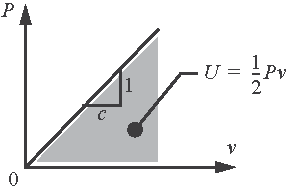
\includegraphics{Figure_13-13.pdf}}{\caption{Elastic response prior to crack growth.}\label{fig13.13}}

\vspace*{-12pt}

Hence,
\begin{align}\label{eq13.26}
G=\frac{1}{t}\left[P \frac{d}{d a}(c P)-\frac{d}{d a}\left(\frac{1}{2} c P^{2}\right)\right].
\end{align}
Performing the differentiations in eq.~(\ref{eq13.26}) we get
\begin{align}\label{eq13.27}
G=\frac{1}{t}\left[P^{2} \frac{d c}{d a}+c P \frac{d P}{d a}-\frac{P^{2}}{2} \frac{d c}{d a}-c P \frac{d P}{d a}\right].\\[-4pt]
\raisebox{4pt}{$\blacktriangle$}\hspace*{-3.6pt}\rule{1pt}{5pt}\hspace*{-0.5pt}\rule{6pc}{1pt}\hspace*{-0.5pt}\rule{1pt}{5pt}\hspace*{-3.8pt}\raisebox{4pt}{$\blacktriangle$}\hspace*{1.1pc}\nonumber\\[-7pt]
\mbox{add to zero}\hspace*{2.5pc}\nonumber
\end{align}
Therefore, the strain energy release rate is independent of whether the load changes or not during crack growth, and we get
\begin{align}\label{eq13.28}
G=\frac{P^{2}}{2 t} \frac{d c}{d a}.
\end{align}
Consider two types of loading as shown in figure~\ref{fig13.14}.

\begin{enumerate}
\item[a.] Load $P= \textrm{constant}$ during crack growth\vspace*{7pt}

\processfigure[!h]{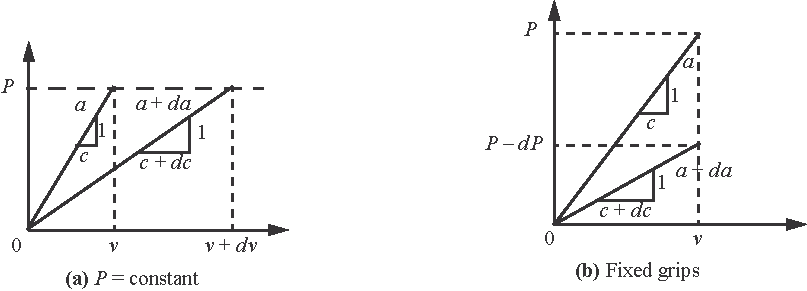
\includegraphics{Figure_13-14.pdf}}{\caption{Two types of loading under mode I crack growth.}\label{fig13.14}}

The strain energy and its differential with respect to the compliance at a fixed value of the load is
\begin{equation*}
U=\left.\frac{1}{2} c P^{2} \quad d U\right|_{P}=\frac{P^{2}}{2} d c,
\end{equation*}
\vspace*{2pt}
\pagebreak

\noindent or
\begin{align}\label{eq13.29}
\left.\frac{1}{t} \frac{d U}{d a}\right|_{P}=\frac{P^{2}}{2 t} \frac{d c}{d a}.
\end{align}
Comparing eq.~(\ref{eq13.28}) and eq.~(\ref{eq13.29}), we find
\begin{align}\label{eq13.30}
G=\left.\frac{1}{t} \frac{d U}{d a}\right|_{P}.
\end{align}
That is, $d U>0$ for $d a>0$, and for $P$ fixed in value.\vspace*{4pt}

\item[b.] Fixed grips with $v = \textrm{constant}$\vspace*{7pt}

In this case $U=\left(c P^{2}\right) / 2=\left(c\left(\frac{v}{c}\right)^{2}\right) / 2=v^{2} /(2 c)$ since $P=v / c$. Hence, the differential of the strain energy with fixed grips is
\begin{align}\label{eq13.31}
\left.d U\right|_{v}=d\left(\frac{v^{2}}{2 c}\right)=\left(\frac{v^{2}}{2}\right)\left(-\frac{d c}{c}\right)=-\frac{1}{2}\left(\frac{v}{c}\right)^{2} d c.
\end{align}
Substitute $v=c P$ for $v$ in eq.~(\ref{eq13.31}) to get
\begin{align}\label{eq13.32}
\left.\frac{1}{t} \frac{d U}{d a}\right|_{v}=-\left(\frac{P^{2}}{2 t} \frac{d c}{d a}\right).
\end{align}
Comparing eq.~(\ref{eq13.28}) and eq.~(\ref{eq13.32}), we find
\begin{align}\label{eq13.33}
G=-\left.\left(\frac{1}{t} \frac{d U}{d a}\right)\right|_{v}.
\end{align}
So $d U<0$ for $d a>0$, and for $v$ fixed in value, and no external work is done by load \textit{P}.
\end{enumerate}

Equations (\ref{eq13.30}) and (\ref{eq13.33}) show that the strain energy release rate is always equal to the derivative of the strain energy apart from the sign. Crack extension occurs when $G_{I}=R$ where \textit{R} is the work of fracture, or the material resistance to crack extension. For an ideally brittle material, like glass, $R \sim 2 \mathrm{~J} / \mathrm{m}^{2}$, which is twice the surface energy to create two new surfaces. For ductile metals, the work of fracture is much larger\vadjust{\vspace*{6pt}\pagebreak} than the surface energy to create new free surfaces because of plastic deformation occurring in front of the crack tip. During crack extension energy is expended by deformation of a new plastic zone at the tip of the advancing crack. Note that the Griffith energy criterion is based on linear elastic material behavior, so the formation of a nonlinear effect such as plasticity seems to negate the analysis. However, if the plastic zone ahead of the crack tip is very small compared to the bulk material remaining elastic, then the criterion is applicable. If the increase in energy required for plastic deformation is independent of the increase in crack area, then $R=\text { constant }$. From fracture tests of a material, the value of \textit{G} at crack growth, which equals \textit{R}, is called the \textbf{critical strain energy release} \textbf{rate}, denoted by $G_{\mathrm{c}}$, and is assumed to be a material parameter.
\begin{gather}
\textrm{If $G<G_{\mathrm{c}}$ no crack growth} \nonumber\\
\textrm{If $G=G_{\mathrm{c}}$ crack growth initiates.} \label{eq13.34}
\end{gather}

\section{Relation between \emph{K} and \emph{G}}\label{sec13.6}

Consider the through-the-thickness crack in a infinite plate of unit thickness subject to uniform tension, or mode I loading.as shown in figure~\ref{fig13.4}. The through-crack opening displacement for a crack length of \textit{2a} is shown in figure~\ref{fig13.5} and given by eq.~(\ref{eq13.12}). The relation between \textit{K} and \textit{G} is established by computing the work done to close a crack of length \textit{2a}, and restore the uniform stress $\sigma$ in the plate to its pre-cracked value. This crack closure method is presented in several texts on fracture mechanics (e.g., Broek (1986, p. 126), Anderson (1995, p. 70), and Sun (1998, p. 164)). The analysis for the crack closure method that follows is from Sun. Denote the work done to close the crack as $W_{s}(a)$ where
\begin{align}\label{eq13.35}
W_{s}(a)=2 \int_{-a}^{a} \frac{1}{2} \sigma v(x) d x.
\end{align}
The factor of 2 preceding the integral in the expression for $W_{s}(a)$ accounts for two crack surfaces. The crack opening displacement $v(x)$ given by eq.~(\ref{eq13.12}) is symmetric with respect to $x$, and $\sigma$ is independent of the displacement. Perform the integration to get the work done to close the crack as
\begin{align}\label{eq13.36}
W_{s}(a)=4 \int_{0}^{a} \frac{1}{2} \sigma v(x) d x=\frac{a^{2} \pi(1+\kappa)(1+v) \sigma^{2}}{4 E}.
\end{align}
The mode I strain energy release rate per crack tip is
\begin{align}\label{eq13.37}
G_{I}=\frac{1}{2} \frac{\partial W_{s}}{\partial a}=\frac{a \pi(1+\kappa)(1+v) \sigma^{2}}{4 E}.
\end{align}
Substitute $\sigma=K_{I}/\sqrt{\pi a}$ from (\ref{eq13.8}), and substitute eq.~(\ref{eq13.13}) for $\kappa$, in the previous equation to get
\begin{align}\label{eq13.38}
G_{I}=\frac{K_{I}^{2}}{E^{\prime}},
\end{align}
where
\begin{align}\label{eq13.39}
E^{\prime}=E \text { for plane stress } \textrm{ and } E^{\prime}=E /(1-v^{2}) \text { for plane strain }.
\end{align}
For mode II fracture the relation between \textit{K}$_\textrm{II}$ and \textit{G}$_\textrm{II}$ is
\begin{align}\label{eq13.40}
G_{I I}=\frac{K_{I I}^{2}}{E^{\prime}}.
\end{align}
\vspace*{3pt}\vspace*{-7pt}
\pagebreak

Equations (\ref{eq13.38}) to (\ref{eq13.40}) are also valid for finite dimensions and arbitrary loading, however, \textit{K}$_\textrm{I}$ and \textit{K}$_\textrm{II}$ depend on the configuration and loading of the plate. Thin plates that are closer to the ideal plane stress condition have higher fracture toughness than thick plates that are closer to the state of plane strain. Most standard fracture tests are performed using thick specimens, and thus they give fracture toughness under the plane strain condition. Fracture toughness of a material can be given by either $G_{c}$ or $K_{c}$.

\subsection{Mixed mode fracture}\label{sec13.6.1}

Generally, crack growth occurs under mixed mode loading. Under this type of loading, crack growth might occur before any of the energy release rate components attain their individual critical value. Failure interaction criteria are established from mixed mode fracture test configurations. The following criterion has been shown to fit test data for many materials quite well:
\begin{align}\label{eq13.41}
\frac{G_{I}}{G_{I c}}+\frac{G_{I I}}{G_{I I c}}=1,
\end{align}
where \textit{G}$_\textit{Ic}$ and \textit{G}$_\textit{IIc}$ are the single mode critical energy release rates for modes I and II, respectively. From the relations between \textit{G} and \textit{K} in eqs. (\ref{eq13.38}) and (\ref{eq13.40}), the previous criterion (\ref{eq13.41}) in terms of the \textbf{stress intensity factors }is
\begin{align}\label{eq13.42}
\left(\frac{K_{I}}{K_{\textit{Ic}}}\right)^{2}+\left(\frac{K_{I I}}{K_{\textit{IIc}}}\right)^{2}=1.
\end{align}

\vspace*{-1pc}

\section{Interlaminar failure in composites: delamination}\label{sec13.7}

The main failure modes of fiber-reinforced polymer (FRP) composites were discussed in article~\ref{sec9.1} on page~\pageref{sec9.1}. Laminated composite structures can fail within lamina, which is intralaminar failure; between lamina, which is interlaminar failure; or by interacting together in a complex manner. Interlaminar failure refers to debonding of adjacent lamina, or delamination, which can initiate from an interfacial crack.

\begin{quote}%
Delamination is the chief vulnerability of composites. However, Boeing's Chief Technology Officer states: ``We designed [composite parts] so they carry loads even if delaminated. We know how to inspect and we know how to repair.'' (Canaday, 2015)
\end{quote}

In this section delamination is analyzed with the concepts from fracture mechanics. An initial delamination crack is postulated and fracture mechanics principles are used to determine if the crack will propagate in a self-similar manner. The examples analyzed here are standard fracture test configurations. The tests are performed on unidirectional composites with the fibers oriented such that they are parallel to the length of the initial delamination. Consequently, the fracture configurations are modeled as laminated beams. The material is carbon fiber-reinforced epoxy with the properties listed in table~\ref{tab13.4}.

\begin{table}[!h]
\processtable{T300/977-2 carbon fiber composite \label{tab13.4}}{%
\tabcolsep=12pt\begin{tabular}{@{}llllll@{}}
\toprule
\colhead{$E_{\textbf{1}}$} & \colhead{$E_{\textbf{1}}$} & \colhead{$\nu_{\textbf{21}}$} & \colhead{$G_{\textbf{12}}$} & \colhead{$G_{\textbf{\textit{Ic}}}$} & \colhead{$G_{\textbf{\textit{IIc}}}$} \\
\midrule
150 GPa & 11.0 GPa & 0.25 & 6.0 GPa & 352 J/m$^{2}$ & 1,450 J/m$^{2}$ \\
\botrule
\end{tabular}}{}
\vspace*{-1pc}
\end{table}

\noindent Note that the critical mode I strain energy release rate \textit{G}$_{\textit{Ic}}$ for interface fracture is the order of the work of fracture listed for epoxy resins in article~\ref{sec13.5} on page~\pageref{sec13.5}\vadjust{\vspace*{6pt}\pagebreak}.

\begin{example*}[Double cantilever beam (DCB) fracture test specimen]\label{ex13.3}Consider a cantilever, laminated beam subject to equal and oppositely directed forces of magnitude $P$ applied at the free end. Under the action of the forces there is a crack at the free end perpendicular to the forces of length $a$ and centered with respect to the depth of the beam. The length of the beam is \textit{L}, depth is \textit{2h,} and its thickness is $t$. This is a case of mode I loading, and the initial crack length $a_{0}=50 \mathrm{~mm}$ when $P=0$. See figure~\ref{fig13.15}. The following data is specified: $h=1.98 \mathrm{~mm}$, $t=20 \mathrm{~mm}$, and $L \gg 2 h$. Material properties are listed in table~\ref{tab13.4}. Let $v$ denote the relative vertical displacement of the load points. Determine static response of the beam and plot it on the \textit{P-v} plane. Analytical and numerical solutions for this example were originally given by Mi, et~al., (1998).

\begin{figure}[!h]
\centerline{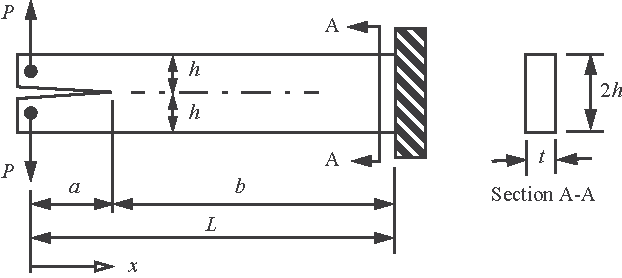
\includegraphics{Figure_13-15.pdf}}
\caption{Double cantilever beam configuration of example~\ref{ex13.3}.}\label{fig13.15}
\vspace*{-0.4pc}
\end{figure}

\subsubsection{Solution.} We use Castigliano's second theorem to determine the relative displacement $v$. Complementary strain energy is stored in each arm of the beam for $0 \leq x \leq a$, and not in the un-stressed section of the beam from $a<x \leq L$. The complementary strain energy is
\begin{equation}
U^{*}=\frac{1}{2} \int_{0}^{a} \frac{M_{1}^{2}}{E I} d x+\frac{1}{2} \int_{0}^{a} \frac{M_{2}^{2}}{E I} d x, \label{eq13.3.a}\tag{a}
\end{equation}
where the bending moment in the upper arm is $M_{1}$, the bending moment in the lower arm is $M_{2}$, and the second area moment of each arm is
\begin{equation}
I=\frac{t h^{3}}{12}=12.9373 \mathrm{~mm}^{4}. \label{eq13.3.b}\tag{b}
\end{equation}
Note that the modulus of elasticity $E=E_{1}$. The distribution of the bending moment in each arm is determined from equilibrium. The results are
\begin{equation}
M_{1}(x)=-M_{2}(x)=-P x \quad 0 \leq x \leq a. \label{eq13.3.c}\tag{c}
\end{equation}
Hence,
\begin{equation}
\nu=\frac{\partial U^{*}}{\partial P}=\frac{1}{E I}\left\{\int_{0}^{a}(-P x)(-x) d x+\int_{0}^{a}(P x)(x) d x\right\}=\frac{2 P}{E I} \int_{0}^{a} x^{2} d x. \label{eq13.3.d}\tag{d}
\end{equation}

\vspace*{-1pc}\pagebreak

\noindent Performing the integration in eq. (\textbf{\ref{eq13.3.d}}) we get
\begin{equation}
v=\frac{2}{3} \frac{P a^{3}}{E I}. \label{eq13.3.e}\tag{e}
\end{equation}
From this last equation, the compliance of the beam is given by $c=(2 a^{3}) /(3 E I)$. The strain energy release rate is determined from eq.~(\ref{eq13.28}), which yields
\begin{equation}
G_{I}=\frac{P^{2}}{2 t} \frac{d c}{d a}=\frac{P^{2} a^{2}}{t E I}. \label{eq13.3.f}\tag{f}
\end{equation}
At the initiation of crack growth $G_{I}=G_{I c}$, so
\begin{equation}
G_{I c}=\frac{P^{2} a^{2}}{t E I} \text { at crack growth }. \label{eq13.3.g}\tag{g}
\end{equation}
Solve eq. (\textbf{\ref{eq13.3.g}}) for the crack length \textit{a} to get
\begin{equation}
a=\left(t E I G_{I c}\right)^{1 / 2}\left(\frac{1}{P}\right). \label{eq13.3.h}\tag{h}
\end{equation}
Substitute eq. (\textbf{\ref{eq13.3.h}}) for crack length $a$ into eq. (\textbf{\ref{eq13.3.e}}) to get
\begin{equation}
v=\frac{2}{3} \frac{\left(t G_{I c} E I\right)^{3 / 2}}{E I P^{2}} \text { for the propagating crack }. \label{eq13.3.i}\tag{i}
\end{equation}

Prior to crack growth eq. (\textbf{\ref{eq13.3.e}}) determines the response as
\begin{equation}
v=\frac{2}{3} \frac{(50 \mathrm{~mm})^{3} P}{\left(150,000 \mathrm{~N} / \mathrm{mm}^{2}\right)\left(12.9373 \mathrm{~mm}^{4}\right)}=(0.04294 \mathrm{~mm} / \mathrm{N}) P. \label{eq13.3.j}\tag{j}
\end{equation}
For the propagating crack eq. (\textbf{\ref{eq13.3.h}}) evaluates to
\begin{equation}
a=\big[(20 \mathrm{~mm})\big(150{,}000 \mathrm{~N} / \mathrm{mm}^{2}\big)\big(12.9373 \mathrm{~mm}^{4}\big)(0.352 \mathrm{~N} / \mathrm{mm})\big]^{1/2}\left(\frac{1}{P}\right)=\frac{3{,}696.19 \textrm{ Nmm}}{P}. \label{eq13.3.k}\tag{k}
\end{equation}
For the initial crack length $a_{0}=50 \mathrm{~mm}$ eq. (\textbf{\ref{eq13.3.k}}) determines the maximum load, and then either eq. (\textbf{\ref{eq13.3.e}}) or eq. (\textbf{\ref{eq13.3.j}}) determines the corresponding displacement; i.e.,
\begin{equation*}
P=73.9238 \mathrm{~N} \textrm{ and } v=3.1744 \textrm{ mm at the initiation of crack growth.}
\end{equation*}
For the propagating crack eq. (\textbf{\ref{eq13.3.i}}) evaluates to
\begin{equation}
v=\frac{2}{3} \frac{[20 \mathrm{~mm}(0.352 \mathrm{~N} / \mathrm{mm})\left(150,000 \mathrm{~N} / \mathrm{mm}^{2}\right)\left(12.9373 \mathrm{~mm}^{4}\right)]^{3 / 2}}{\left(150,000 \mathrm{~N} / \mathrm{mm}^{2}\right)\left(12.9373 \mathrm{~mm}^{4}\right)}\left(\frac{1}{P^{2}}\right)=17,347.4 \mathrm{~N}^{2} \mathrm{~mm}\left(\frac{1}{P^{2}}\right). \label{eq13.3.l}\tag{l}
\end{equation}
Equations (\textbf{\ref{eq13.3.j}}) and (\textbf{\ref{eq13.3.l}}) are used to plot the load-displacement response shown in figure~\ref{fig13.16}.

\processfigure{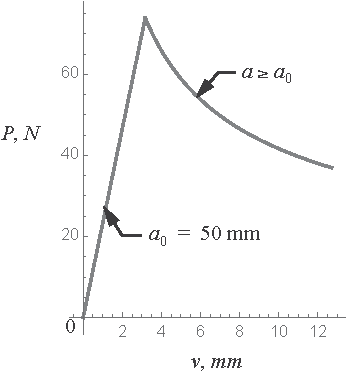
\includegraphics{Figure_13-16.pdf}}{\caption{Static response of the DCB configuration. Crack growth begins at 73.92~N and 3.17~mm.}\label{fig13.16}}

In load control, where \textit{P} is specified and increased slowly from zero, a sudden dynamic increase in crack growth occurs at $P=73.9238 \mathrm{~N}$ since there is no stable adjacent equilibrium state. In displacement control, where $v$ is specified and is increased slowly from zero to 3.17~mm, the load \textit{P} increases to 73.92~N. For $v>3.17 \mathrm{~mm}$ the load decreases as the crack increases in length.\hfill$\blacksquare$
\end{example*}
\vspace*{2pt}
\pagebreak

\begin{example*}[End load split (ELS) configuration]\label{ex13.4}The end load split (ELS) configuration shown in figure~\ref{fig13.17} has an initial crack length denoted by $a=a_{0}$, length by $L$, height by $2 h$, and thickness normal to the \textit{x-y} plane by $t$. The lower arm at the tip is subject to vertical force $P$. Both arms below and above the crack are identical and are subject to the same load as shown in the free body diagrams of figure~\ref{fig13.18}. Hence, both arms have the same lateral displacement $v(x)$ and rotation $-v^{\prime}(x)$. The\break $x$-direction displacement at the crack tip of the upper arm is $\frac{h}{2}\left[v^{\prime}(a)\right]$, and the $x$-direction displacement of\break the lower arm at the crack tip is $\frac{h}{2}\left[-v^{\prime}(a)\right]$, Thus, the relative axial displacement between the lower surface of the upper arm and the upper surface of the lower arm is $h\left[v^{\prime}(a)\right]$, which is a mode II displacement loading. Determine the strain energy release rate \textit{G}$_\textrm{II}$. Analytical and numerical solutions for this example were originally given by Chen et al. (1999).

\begin{figure}[!h]\vspace*{-6pt}
\centerline{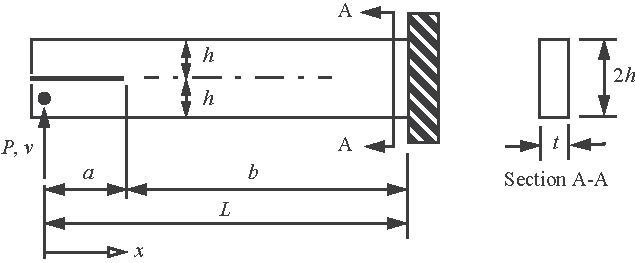
\includegraphics{Figure_13-17.pdf}}
\caption{End load split configuration of example~\ref{ex13.4}.}\label{fig13.17}
\end{figure}

\subsubsection{Solution.} The strain energy is
\begin{equation}
U=\int_{0}^{a} \frac{M_{1}^{2}}{2 E I} d x+\int_{0}^{a} \frac{M_{2}^{2}}{2 E I} d x+\int_{a}^{L} \frac{M_{3}^{2}}{2 E(8 I)} d x, \label{eq13.4.a}\tag{a}
\end{equation}
where $\textit{M}_1$ denotes the bending moment in the arm below the crack, $\textit{M}_2$ the bending moment in the arm above the crack, and $\textit{M}_3$ the bending moment in the segment not containing the crack. The second area moment of\vadjust{\vspace*{6pt}\pagebreak} each arm is denoted by \textit{I}, and $I=\left(t h^{3}\right)/12$. From the free body diagrams shown in figure~\ref{fig13.18}, equilibrium determines the bending moments as
\begin{gather}
M_{1}(x)=M_{2}(x)=-\left(\frac{P}{2}\right) x \quad 0 \leq x \leq a, \textrm{ and} \label{eq13.4.b}\tag{b}\\
M_{3}(x)=-(x-a) P+M_{1}(a)+M_{2}(a)=-P x \quad a \leq x \leq L.  \label{eq13.4.c}\tag{c}
\end{gather}
Substitute eqs. (\textbf{\ref{eq13.4.b}}) and (\textbf{\ref{eq13.4.c}}) for the bending moments in eq. (\textbf{\ref{eq13.4.a}}), and perform the integrations to get
\begin{equation}
U=\frac{(3 a^{3}+L^{3})P^{2}}{48 E I}. \label{eq13.4.d}\tag{d}
\end{equation}
The mode II strain energy release rate is
\begin{equation}
G_{II}=\frac{\partial U}{t \partial a}=\frac{3 a^{2} P^{2}}{16 t E I}.\label{eq13.4.e}\tag{e}
\end{equation}\hfill\qed
\end{example*}

\begin{figure}[!t]
\centerline{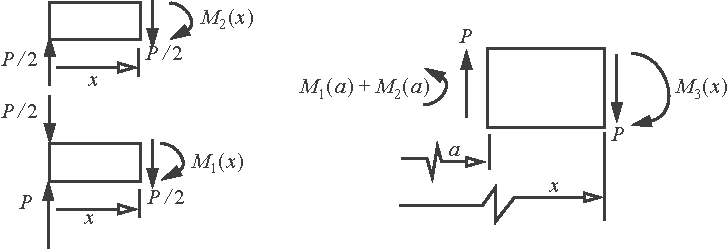
\includegraphics{Figure_13-18.pdf}}
\caption{Free body diagrams of the three segments of the ELS configuration.}\label{fig13.18}
\end{figure}

\vspace*{-1pc}

\subsection{Mixed mode fracture}\label{sec13.7.1}

Consider a cantilever beam of length \textit{L} containing a through crack of length $a$ centered at its free end. This configuration subject to load \textit{P} shown in part (a) of figure~\ref{fig13.19} is labeled FRMM, which means fixed ratio mixed mode. By the method of superposition FRMM is equivalent to the DCB test configuration shown in part (b) of the figure plus the ELS test configuration shown in part (c) of the figure. Hence, the FRMM configuration is a mixed mode I and II fracture test.

\processfigure{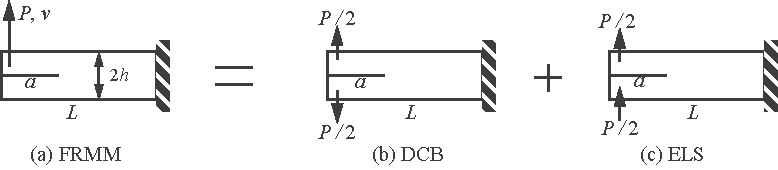
\includegraphics{Figure_13-19.pdf}}{\caption{Mixed mode I and II loading: (a) fixed ratio mixed mode, (b) double cantilever beam, and (c) end load split.}\label{fig13.19}}
\vspace*{-5pt}
\pagebreak

From eq. (\textbf{\ref{eq13.3.f}}) in example~\ref{ex13.3} the mode I strain energy release rate for the configuration in part (b) of figure~\ref{fig13.19}~is
\begin{align}\label{eq13.43}
G_{I}=\left.\frac{P^{2} a^{2}}{t E I}\right|_{P \rightarrow P / 2}=\frac{P^{2} a^{2}}{4 t E I}.
\end{align}
From eq. (\textbf{\ref{eq13.4.e}}) in example~\ref{ex13.4} the mode II strain energy release rate for the configuration in part (c) of figure~\ref{fig13.19}~is
\begin{align}\label{eq13.44}
G_{I I}=\frac{3 a^{2} P^{2}}{16 t E I}.
\end{align}
Therefore, the mixed mode ratio for the FRMM configuration is $G_{I}/G_{I I}=4/3$.

\begin{example}[Response of the FRMM configuration shown in figure~\ref{fig13.19}]\label{ex13.5}Take the height of the arms $h=1.5 \mathrm{~mm}$, thickness $t=10 \mathrm{~mm}$, length $L=100 \mathrm{~mm}$, so that $I=2.8125 \mathrm{~mm}^{4}$. The initial crack length $a_{0}=40 \mathrm{~mm}$. From table~\ref{tab13.4} where $E=150{,}000 \mathrm{~N} / \mathrm{mm}^{2}$, $G I_{c}=0.352 \mathrm{~N} / \mathrm{mm}$ and $G I I_{c}=1.45 \mathrm{~N} / \mathrm{mm}$. Determine the load-displacement response, and the crack-length-displacement response.

\subsubsection{Solution.} The bending moment in the FRMM configuration is $M=-P x$, $0 \leq x \leq L$. The strain energy is
\begin{equation}
U=\int_{0}^{a} \frac{M^{2}}{2 E I} d x+\int_{a}^{L} \frac{M^{2}}{2 E(8 I)} d x=\frac{\left(7 a^{3}+L^{3}\right) P^{2}}{48 E I}, \label{eq13.5.a}\tag{a}
\end{equation}
where $I=t h^{3} / 12$. The displacement corresponding to load \textit{P} is given by
\begin{equation}
v=\frac{\partial U}{\partial P}=\frac{(7 a^{3}+L^{3})P}{24 E I}. \label{eq13.5.b}\tag{b}
\end{equation}
The displacement prior to crack growth
\begin{equation}
v=v_{0}=(0.143012 \mathrm{~mm} / \mathrm{N}) P. \label{eq13.5.c}\tag{c}
\end{equation}
The mode I (\ref{eq13.43}) and mode II (\ref{eq13.44}) strain energy release rates are
\begin{equation}
G_{I}=\left[5.92593 \times 10^{-8}\left(\frac{1}{\mathrm{~mm}^{3} N}\right)\right] a^{2} P^{2} \quad G_{I I}=\left[4.44444 \times 10^{-8}\left(\frac{1}{\mathrm{~mm}^{3} N}\right)\right] a^{2} P^{2}. \label{eq13.5.d}\tag{d}
\end{equation}
Evaluate the mixed mode fracture criterion (\ref{eq13.41}) to get
\begin{equation}
\left[1.99002 \times 10^{-7}\left(\frac{1}{\mathrm{~mm}^{2} N^{2}}\right)\right] a^{2} P^{2}=1. \label{eq13.5.e}\tag{e}
\end{equation}
Solve eq.~(\textbf{\ref{eq13.5.e}}) for \textit{a} to find
\begin{equation}
a=\frac{2241.67 \textrm{ mmN}}{P}. \label{eq13.5.f}\tag{f}
\end{equation}
Substitute the crack length from eq. (\textbf{\ref{eq13.5.f}}) into eq. (\textbf{\ref{eq13.5.b}}) to get the displacement for the propagating crack
\begin{equation}
v=\frac{7{,}797.87 \textrm{ mmN}^{2}}{P^{2}}+(0.0987654 \mathrm{~mm} / \mathrm{N}) P. \label{eq13.5.g}\tag{g}
\end{equation}
\vspace*{2pt}\vspace*{-8pt}
\pagebreak

\noindent The transition from the initial crack to the propagating crack is obtained by equating eq. (\textbf{\ref{eq13.5.c}}) to eq. (\textbf{\ref{eq13.5.g}}). The result~is
\begin{equation}
(v, P)=(8.01466 \mathrm{~mm}, 56.04 \mathrm{~N}). \label{eq13.5.h}\tag{h}
\end{equation}
For the crack length $a=L$, eq. (\textbf{\ref{eq13.5.f}}) yields $P=22.41 \mathrm{~N}$. Hence, at completed separation
\begin{equation}
(v, P)=17.32 \mathrm{~mm}, 22.41 \mathrm{~N}. \label{eq13.5.i}\tag{i}
\end{equation}
The response plots for the FRMM fracture specimen are shown in figure~\ref{fig13.20}.
\end{example}

\processfigure{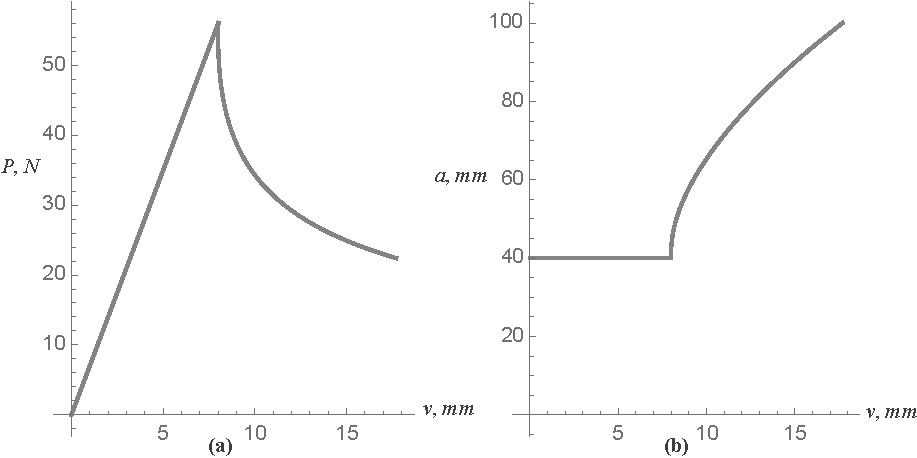
\includegraphics{Figure_13-20.pdf}}{\caption{(a) Load-displacement, and (b) crack length vs. displacement for the FRMM facture test.}\label{fig13.20}}

\begin{thebibliography}{}\label{sec13.8}
\bibitem{} Anderson, T.L. \textit{\textbf{Fracture Mechanics}}, 2d ed. Boca Raton, FL: CRC Press, Inc., 1995.

\bibitem{} Broek, David. \textbf{Elementary Engineering Fracture Mechanics}, 4d ed., Dordrecht, The Netherlands: Martinus Nijhoff Publishers, 1986, p. 126.

\bibitem{} Canaday, H. ``Composites vs. Metals.'' \textit{\textbf{Aerospace America}}, May 2015, p. 18.

\bibitem{} Cawthon, Bill. ``De Havilland's Comet: The Original Jetliner.'' Promotex Online, June 15, 2005, \url{http://www.promotex.ca/articles/cawthon/2005/2005-06-15_article.html}.

\bibitem{} Chen, J., M. Crisfield, A. Kinloch, E. Busso, E., F. Matthews, and Y. Qiu. ``Predicting Progressive Delamination of Composite Material Specimens via Interface Elements.'' \textit{\textbf{Mechanics of Composite Materials and Structures}} 6, (1999): 301--317.

\bibitem{} Dowling, Norman. \textit{\textbf{Mechanical Behavior of Materials: Engineering Methods for Deformation, Fracture and Fatigue}}, 2d ed. Upper Saddle River, NJ: Prentice Hall, 1999, pp. 291, 292\vadjust{\vspace*{6pt}\pagebreak}.

\bibitem{} Gordon, J. E. \textit{\textbf{Structures} \textbf{or Why Things Don’t Fall Down}}. Boston: Da Capo Press, 2003. (Originally published by Harmondsworth: Penguin Books, 1978.)

\bibitem{} Kanninen, Melvin F., and Carl H. Popelar. \textit{\textbf{Advanced Fracture Mechanics}}. New York: Oxford University Press, 1985.

\bibitem{} Mi, Y., M. Crisfield, G. Davies, and H-B. Hellweg.``Progressive Delamination Using Interface Elements.'' \textit{\textbf{Journal of Composite Materials}} 332 (1998): 1246--1273.

\bibitem{} Sun, C. T. \textbf{\textit{Mechanics of Aircraft Structures}}. New York: John Wiley \& Sons, 1998.

\bibitem{} ``de Havilland Comet.'' Wikipedia, \url{https://en.wikipedia.org/wiki/De_Havilland_Comet} (accessed February 2008).
\end{thebibliography}

\section{Practice exercises}\label{sec13.9}

\begin{exercise}
\begin{enumerate}[\textbf{2.}]
\item[\textbf{1.}] A monococque fuselage consists of a circular cylindrical shell with a mean radius $\textit{R}=50.0$~in. and wall thickness denoted by $t$, where $R\gg t$. It is subject to internal pressure $p$, with the design ultimate pressure specified as $p= 18.2$~psi. A damage tolerance philosophy allows for the presence of a subcritical crack that will not grow to critical length between periodic inspections. Assume an axial crack through the thickness of the wall of the shell with a length $2a = 2.0$~in. \textbf{Determine the minimum thickness of the shell such that crack growth does not occur at the design ultimate pressure.} The material is 2024-T351 aluminum alloy with a fracture toughness $K_{I c}=31 \textrm{ ksi} \sqrt{\mathrm{in.}}$, and a yield strength of 47~ksi.

\smallskip

The mode I stress intensity factor for an axial crack through the thickness of a cylindrical shell subject to internal pressure is (Anderson, p. 636)
\begin{equation}
K_{I}=\sigma_{\theta} \sqrt{\pi a} \sqrt{1+0.52 \chi+1.29 \chi^{2}-0.074 \chi^{3}}, \label{eq13.6.a}\tag{a}
\end{equation}
where the dimensionless parameter $\chi=a /(\sqrt{R t})$. The circumferential normal stress, or hoop stress, is $\sigma_{\theta}=(p R) / t$.


\item[\textbf{2.}] Consider the cross section at the root of the wing spar in example~\ref{ex6.6} on page~\pageref{ex6.6} as shown in figure~\ref{fig13.21}.

\processfigure[!h]{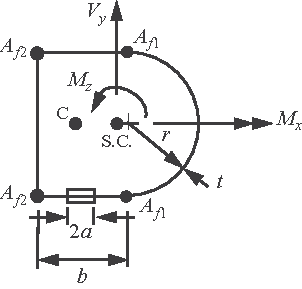
\includegraphics{Figure_13-21.pdf}}{\caption{Cross section at the root of the wing spar in Exercise~~\break 8.2.}\label{fig13.21}}

\noindent During an inspection a one-inch crack ($2a=1.0$) is detected that is parallel to the chord in the center of the lower web at the root section. (This web is labeled branch 4 in Fig.~\ref{fig3.24} on page~\pageref{fig3.24}.) At the root cross section the transverse shear force $V_{y}$, bending moment $M_{x}$, and torque $M_{z}$ are given by
\begin{equation}
V y=\frac{L}{2} \quad M_{x}=\frac{-2 L z_{m a x}}{3 \pi} \quad M_{z}=\frac{e L}{2}. \label{eq13.6.b}\tag{b}
\end{equation}
\vspace*{2pt}\vspace*{-8pt}
\pagebreak

\noindent The total lift force acting on the airplane is denoted by $L$, the span of the wing spar by $z_{\textrm{max}}$, and $e$ denotes the distance from the shear center to the line of action of the lift force acting on the wing. Take $z_{\textrm{max}} = 120$.~in.
Pertinent data are listed in table~\ref{tab13.5}.

\begin{table}[!h]
\processtable{Data from example~\ref{ex6.6} \label{tab13.5}}{%
\tabcolsep=12pt\begin{tabular}{@{}ll|ll@{}}
\toprule\\[-15.5pt]
& & \\[-6pt]
$r$, nose web radius & 6.0 in & $I_{xx}$, second area moment about the $x$-axis & 101.619 in.$^{4}$ \\
$b$, length horizontal web & 7.0 in. & $A_{\textrm{c}}$, area enclosed by the contour & 140.549 in.$^{2}$ \\
$t$, wall thickness & 0.030 in. & $e = X_{\textrm{L}}- X_{\textrm{SC}}$ & 3.604 in. \\[-3pt]
& & \\[-3.5pt]
\botrule
\end{tabular}}{}
\vspace*{-1pc}
\end{table}

To aid in computing the shear stress, the shear flow in the lower web is given by
\begin{equation}
q_{4}\left(s_{4}\right)=\frac{M_{z}}{2 A_{c}}-F_{y 4}\left(s_{4}\right) V_{y}. \label{eq13.6.c}\tag{c}
\end{equation}
Repeating eq. (\textbf{ae}) in example~\ref{ex3.4} on page~\pageref{ex3.4}, the shear flow distribution function is
\begin{equation}
F_{y 4}\left(s_{4}\right)=0.00542827-0.00177133 s_{4} \quad 0 \leq s_{4} \leq 7 \textrm{ in}. \label{eq13.6.d}\tag{d}
\end{equation}
The critical mode I stress intensity factor $K_{I c}=31 \textrm{ ksi} \sqrt{\mathrm{in.}}$, and the critical mode II stress intensity factor $K_{I I c}=23.5 \textrm{ ksi} \sqrt{\mathrm{in}}$. \textbf{Determine the lift force \textit{L} to initiate crack growth using a factor of safety FS~$=$~1.5.}

\item[\textbf{3.}]  Consider the end load split (ELS) fracture configuration in example~\ref{ex13.4} on page~\pageref{ex13.4}. It is modeled as a laminated beam made of unidirectional plies of the carbon-epoxy listed in table~\ref{tab13.4}. Take $\textit{E}_1$ for the modulus of elasticity. For $a_{0}=30 \mathrm{~mm}$, $L=100 \mathrm{~mm}$, $t=30 \mathrm{~mm}$, and $h=1.5 \mathrm{~mm}$, complete the following steps:
\begin{enumerate}[b)]
\item[{\hskip13pt}a)] Use Castigliano's second theorem to determine the tip displacement $v$ at the point of load application.
\item[{\hskip13pt}b)] Determine the crack length $a$ for $G_{I I}=G_{I I c}$.
\item[{\hskip13pt}c)] Determine the displacement $v$ for the crack length in part (b).
\item[{\hskip13pt}d)] Plot the load \textit{P} versus displacement $v$ for $a_{0} \leq a \leq L$. Comment on the \textit{P-v} plot for the propagating crack as compared to the same plot for the DCB configuration shown in figure~\ref{fig13.16}.
\end{enumerate}
Partial answer: The maximum load is 571.183 N.

\item[\textbf{4.}] Consider the fixed ratio mixed mode (FRMM) fracture configuration in article~\ref{sec13.7.1}. It is modeled as a laminated beam of made of unidirectional plies of the carbon-epoxy listed in table~\ref{tab13.4}. Take $E_1$ for the modulus of elasticity. For $a_{0}=40 \mathrm{~mm}$, $L=100 \mathrm{~mm}$, $t=10 \mathrm{~mm}$, and $h=1.5 \mathrm{~mm}$, complete the following steps:
\begin{enumerate}[b)]
\item[{\hskip13pt}a)] Use Castigliano's second theorem to determine the tip displacement $v$ at the point of load application.
\item[{\hskip13pt}b)]  Determine the crack length $a$ from eq.~(\ref{eq13.41}).
\item[{\hskip13pt}c)]  Determine the displacement $v$ for the crack length in part (b).
\item[{\hskip13pt}d)]  Plot the load \textit{P} versus displacement $v$ for $a_{0} \leq a \leq L$.
\end{enumerate}
Partial answer: The maximum load is 56.04~N.
\end{enumerate}
\end{exercise}


\end{document} 